% FEBRUARI 2020, gemaakt door de TeXniCie met een stukje overgenomen uit de bachelorscriptiepresentatie van Freek Geerligs
% kleine aanpassingen gedaan in maart 2023 door de TeXniCie

\documentclass{beamer}

% Packages:
%\usepackage[a4paper]{geometry} 
\usepackage[dutch]{babel} 		% Juiste afbreekregels en dergelijke!
\usepackage{%
	parskip, 					% alinea's (geen indent, regel ertussen)
	amsmath, amssymb,			%
	textcomp,amsthm, 			% Wiskundige symbolen e.d.
	color, 						% Kleuren
	enumerate,					% Voor opsommingen
	hyperref,					% klikbare references/urls in pdf
	graphicx,					% Voor invoegen van plaatjes
	caption,
	%subcaption,
	%subfig,
	mathrsfs,
	amsthm, 						% Definitie,proof, etc environments		
	tikz-cd						% Voor commutatiediagrammen
	}

%%%%%%%%%%%%%%%%%%%%%%%%%%%%%%%%%%%%%

%hieronder opmaak om stellingen mooi te kunenn weergeven en numeren
\theoremstyle{definition}
\newtheorem{dfn}{Definition}[section]% nummering van definities volgt nu met secties
\theoremstyle{example}
\newtheorem{conseq}[dfn]{Consequence}
\newtheorem{const}[dfn]{Construction}
%\theoremstyle{plain}
\newtheorem{thm}[dfn]{Stelling}% nummering van stellingen loopt nu samen met dfn (als [dfn] aan het eind zou staan, zou het een nieuw getal erachter betekenen)
%\newtheorem{lemma}[dfn]{Lemma}
%\newtheorem{example}[]{Example}
%\newtheorem{nexample}[example]{Non-example}

%%%%%%%%%%%%%%%%%%%%%%%%%%%%%%%%%%%%%%%%%

% De layout van de presentatie (kleuren etc), a-eskwadraat heeft een thema maar hieronder kan je ook een andere kiezen.

\usetheme{aes2}
%\usetheme{Frankfurt} %Een ander thema als je deze niet wil gebruiken
%\usecolortheme{dolphin} %crane of dolphin
%\useinnertheme{circles}
%\useoutertheme{smoothbars}

%%%%%%%%%%%%%%%%%%%%%%%%%%
% Pas aan naar je eigen presentatie:
\title{Titel van je presentatie}
\date{Jouw datum hier, bijvoorbeeld \today}
\author{Jouw naam hier}

\begin{document}

\begin{frame}
\titlepage
\end{frame}	

\begin{frame}{Inhoud}% elke slide (met naam tussen {} ) zit in de frame omgeving
	\tableofcontents
\end{frame}

\section{Eerste onderwerp}
% De structuur (sections, subsections e.d.) zoals je die gewend bent in TeX-files kan je nogsteeds gebruiken en heeft invloed op de voortgang die je bij elke slide nu bovenaan ziet verschijnen.


\begin{frame}
	\frametitle{Wat iedereen moet weten voor ik begin}
	Zodra je in de frame-omgeving bent kan je doen wat je gewend bent in \LaTeX. Je kan ook mooie formules invoegen zoals
	\begin{align}
	E &= \frac{p^2}{2m}\\
	E_{rel}^2 &= m^2c^4 + p^2c^2
	\end{align}
	\begin{block}{Belangrijk}
		Het is   B E L A N G R I J K   om op \textit{verschillende} \emph{manieren} \textbf{nadruk} te kunnen leggen!
	\end{block}
 
\end{frame}

\begin{frame}{We gaan verder}
Soms is het jammer als alles wat je wilde zeggen er al staat.\newline
\begin{thm}
	Je weet het bewijs van deze stelling nog niet.
\end{thm}
\begin{block}{Bewijs}
	Het bewijs komt hier.
\end{block}
Maar daar is een oplossing voor...

Laten we dit opnieuw proberen.

\end{frame}

\subsection{Deze subsection komt niet bovenin te staan, maar wel in de inhoudsopgave!}

\begin{frame}{Opnieuw!}
\begin{thm}
	Je weet het bewijs van deze stelling nog niet.
\end{thm}
\pause
\begin{block}{Bewijs}
	Het bewijs komt hier.
\end{block}
\pause
Veel mooier!
\end{frame}

\begin{frame}{Voor gevorderden}
	Nog ingewikkelder in de code:
	\only<1->{We kunnen zelfs tekst ook weer laten verdwijnen. (Of een belangrijk stuk laten staan op de slide.)\\}
	\only<2-3>{Kiekeboe!\\}
	\only<3>{Wie niet weg is is gezien!}
	\only<4->{En door...}
\end{frame}

\begin{frame}
Ook opsommingen kunnen mooier zijn op deze manier
\begin{itemize}
	\only<1-4>{\item 1...}
	\only<2-4>{\item 2...}
	\only<3-4>{\item 3...}
	\only<4>{\item 4, 5, 6, 7, 8}
	\only<5-6>{\item 9...}
	\only<6>{\item 10!}
	\only<7>{\item Ik kom!}
\end{itemize}

\end{frame}

%\begin{frame}{Voor de meer gevorderden, overgenomen uit de  bachelor scriptiepresentatie van Freek Geerligs}
%
%\begin{columns}[T] % align columns
%	\uncover<6->{	\begin{column}{.48\textwidth}
%			\begin{dfn}
%				For $x,y\in \hat R$, we define 
%				the \textbf{Kuratowski-tuple } $(x,y)$ as
%				$$(x,y):=\big\{\{x\},\{x,y\}\big\}$$ 
%			\end{dfn}
%	\end{column}}%
%	
%	\begin{column}{.48\textwidth}
%		
%	\begin{block}{The superstructure}
%	\begin{itemize}
%		\item			$R_0:=\mathbb R$. 
%		\item			$R_{n+1}:=\mathcal P(\bigcup\limits_{k=0}^nR_{k}),$ 
%		\item			$\hat R:= \bigcup\limits_{n\in\mathbb N} R_n$.
%	\end{itemize}
%\end{block}
%	\end{column}%
%	\hfill%
%
%
%\end{columns}
%\pause
%\begin{align*}
%	\uncover<3->{0,1,2 & \in }R_0	=\mathbb R
%	\\
%\uncover<4->{	\mathbb N, \mathbb Z, \mathbb Q, \mathbb R,\{0\},\{0,1\}&\in }R_1	=\mathcal P(\mathbb R)
%	\\ 
%\uncover<5->	{\mathcal T_{eucl}, \big\{\{0\},\{0,1\}\big\}&\in} R_2 =\mathcal P(\mathbb R\cup \mathcal P(\mathbb R))
%	\\
%\uncover<7->	{   \mathbb R^2, \{(x,x+1)|x\in\mathbb R \}, \{(x,y)|x\leq y\}&\in }R_3 =\mathcal P(R_0\cup R_1\cup R_2)
%\\
%\uncover<8->	{  C^\infty(\mathbb R), \mathbb R^\mathbb R, \mathbb R^\mathbb N&\in }R_4 =\mathcal P(R_0\cup R_1\cup R_2\cup R_3)\end{align*}
%
%
%\end{frame}




\section{Toepassingen}
\begin{frame}
\begin{columns}[T]
	\begin{column}[T]{5cm}
		We kunnen ook kolommen naast elkaar maken.
		
		\begin{block}{Ook leuk}
			Met nog meer structuur in de code.
		\end{block}
		\begin{alertblock}{Attentie!}
			Een blok voor nog nog nog meer \emph{nadruk}!
			
			In een net iets andere kleur.
		\end{alertblock}
	\end{column}
	\begin{column}[T]{5cm}
		Zelfs met een plaatje erin!
		\begin{figure}
			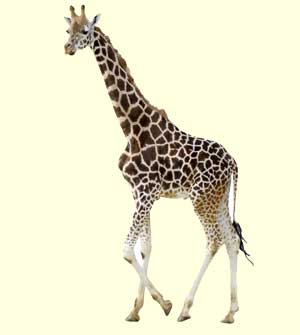
\includegraphics[scale=0.4]{Giraffe_klein.jpg}
			\caption{Een ingevoegd plaatje wat je misschien herkent.}
		\end{figure}
		
	\end{column}
\end{columns}
\end{frame}


\section{Verder}


\begin{frame}{Verder}
Vergeet niet om genoeg te compileren, de inhoudsopgave en de voortgangsbalk gaan niet meteen in \'e\'en keer goed.

Aan het einde van een presentatie bedank je je publiek en je begeleider en laat je ruimte voor het stellen van vragen.

Daarna ben je klaar met je presentatie!
\end{frame}

\begin{frame}{P.S.}
	Het ziet er best wel wat professioneler uit om de a-eswiggle niet bij elke slide in de rechteronderhoek te hebben.
	Hoe je dit doet staat in de code. %zie de preamble, stukje van de layout.
\end{frame}
\end{document}